\documentclass[12pt]{report}

\usepackage[a4paper]{geometry}
\usepackage[utf8]{inputenc}
\usepackage[portuguese]{babel}
\usepackage{graphicx}

\newcommand\tab[1][0.5cm]{\hspace*{#1}}

\title{Projeto de Sistemas Operativos (MiEI) \\ 2017/2018}
\author{Alexandre Mendonça Pinho (a82441) \and Joel Filipe Esteves Gama (a82202) \and Tiago Martins Pinheiro (a82491)}
\date{\today}

\begin{document}
\maketitle

\tableofcontents

\chapter{Introdução}
\label{sec:introducao}

\tab Neste projeto é-nos proposto construir um sistema para processamento de notebooks, que misturam fragmentos de código, resultados da execução, e documentação. Estes notebooks, tratam-se de ficheiros de texto, que depois de processados, são modificados de modo a incluir resultados da execução de código ou comandos nele embebidos.

\chapter{Descrição do projeto}
\label{sec:descricao}

\chapter{Exemplo}
\label{sec:exemplo}

Ficheiro de input exemplo:

\texttt{
\newline
    Listagem da diretoria atual\newline
    \$ ls\newline
\newline
    O número de ficheiros na listagem\newline
    \$ | wc -l\newline
\newline
    O nome do primeiro elemento\newline
    \$ 2 | head -1\newline
\newline
    Aceitar input do utilizador\newline
    \$ cat
}

\begin{figure}
    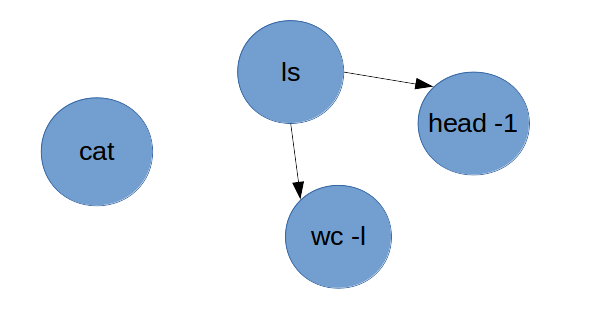
\includegraphics[width=\linewidth]{grafo_execucao_exemplo.png}
    \caption{Grafo de execução}
    \label{fig:grafo_execucao}
\end{figure}

\begin{figure}
    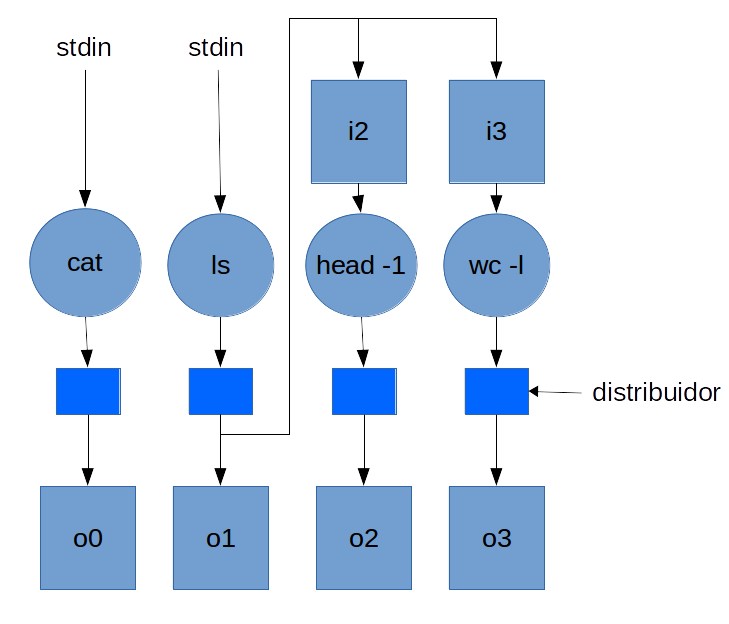
\includegraphics[width=\linewidth]{esquema_execucao_exemplo.png}
    \caption{Esquema de execução}
    \label{fig:esquema_execucao}
\end{figure}

\noindent Ficheiro de output resultante, ao introduzir pelo no teclado o string "Hello, world!\textbackslash n":

\texttt{
\newline Listagem da diretoria atual
\newline \$ ls
\newline >>>
\newline distribuidor \newline distribuidor.c \newline i1 \newline i2
\newline include \newline lib \newline main.c \newline Makefile
\newline notebook \newline o0 \newline o1 \newline o2 \newline o3
\newline obj \newline README.md \newline relatorio \newline test
\newline <<<
\newline O número de ficheiros na listagem
\newline \$ | wc -l
\newline >>>
\newline 17
\newline <<<
\newline O nome do primeiro elemento
\newline \$ 2 | head -1
\newline >>>
\newline distribuidor
\newline <<<
\newline Aceitar input do utilizador
\newline \$ cat
\newline >>>
\newline Hello, world!
\newline <<<
\newline
}

\chapter{Conclusão}
\label{sec:conclusao}

\end{document}
